
		\begin{tcolorbox}[colback=blue!5!white,colframe=blue!75!black,title=I2C]
			Es un puerto y protocolo de comunicación serial, define la trama de datos y las conexiones físicas para transferir bits entre 2 dispositivos digitales. El puerto incluye dos cables de comunicación, SDA (Datos seriales) y SCL (reloj serial). Además el protocolo permite conectar hasta 127 dispositivos esclavos con esas dos líneas, con hasta velocidades de 100, 400 y 1000 kbits/s. \end{tcolorbox}
Para comenzar con las pruebas lo primero que se realizó es la conexión de diversos sensores en una protoboard. Se generó un programa de Arduino dónde a través de I2C se realizaba la comunicación. \\ Conjuntamente con estos sensores de Presión, Humedad y Temperatura se utilizó un sensor para medir presión diferencial, para digitalizar estos datos valores se utilizó un convertidor analógico digital.\\
Este primer prototipo se utilizó para comparar los datos de presión, temperatura y humedad con los valores obtenidos con los dispositivos calibrados con los que cuenta el laboratorio.
Como paso siguiente se eligieron los sensores con menos fluctuaciones y se armó una placa para que no se desconecten.
\\
Los elementos que se decidió utilizar fueron los siguientes:
\begin{itemize}
	\item  \textbf{BME280:} Sensor de presión atmosférica, temperatura y humedad relativa.
	\item \textbf{SI7021:} Sensor de temperatura y humedad relativa.
	\item \textbf{MPXV7002:} Sensor de presión diferencial.
	\item \textbf{ADS1115:} Convertidor analógico digital 16bits.
\end{itemize}	

\begin{figure}[htb]
	\centering
	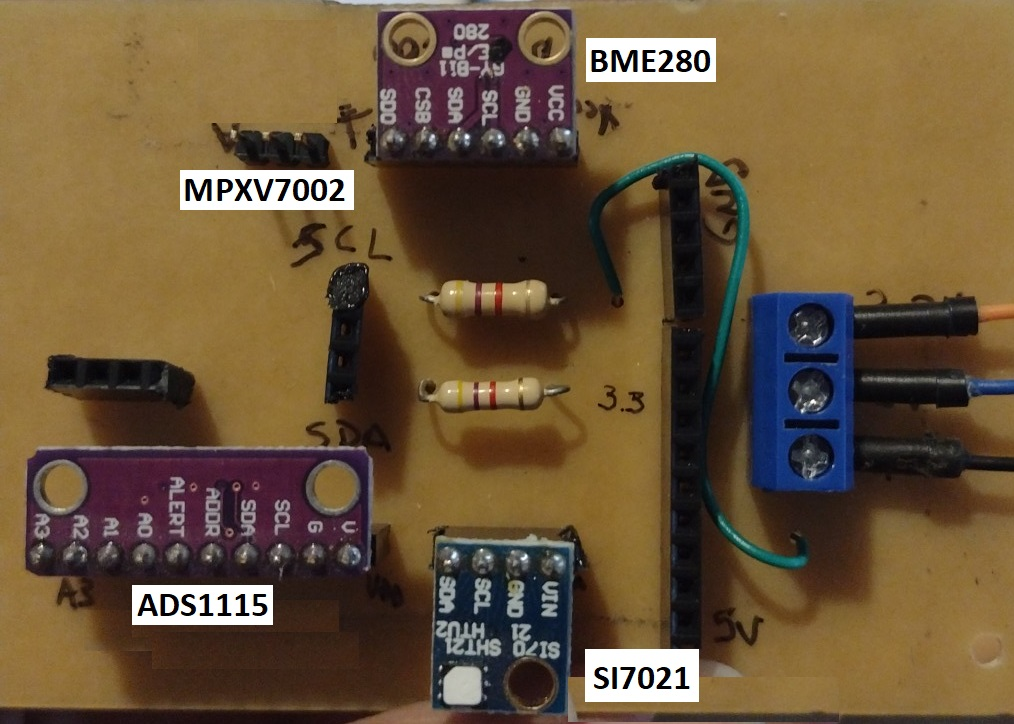
\includegraphics[scale=0.2]{sensores.jpg}
	\captionof{figure}{Placa con sensores}
	\label{fig:sensoresa}
\end{figure}

\subsection{Ecuación velocidad del aire}
El Laboratorio de Mecánica de Fluidos, antes de comenzar con este proyecto utilizó un archivo Excel para hacer la corrección de la velocidad del aire. En este se calcula matemáticamente la densidad del aire en función de la presión, temperatura y humedad atmosférica. Esta ecuación fue desarrollada dentro del programa de Arduino para observar como dato final la velocidad del aire.

	%	densidad_funcion_P_T_H.pdf  dentro del drive


    \subsection{Programa Arduino}
        \subsubsection{Ecuación velocidad del aire}
	%	densidad_funcion_P_T_H.pdf  dentro del drive
    \subsection{Pruebas}
    aca explicar que se hizo sin filtros y porq se filtro despues
        \subsubsection{Filtros}
        que filtro se utilizo y porq y cuando
    - Poner donde se agrego.

\newpage